\section{Introduction}
Schroedinger's equation for two electrons in a three-dimensional harmonic osillator well


\section{Task 02a}
Mathematical intermezzo: A unitary transformation preserves the orthogonality of the obtained eigenvectors. We assume the basis is orthogonal:
$\mathbf{v_j^Tv_i} = \delta_{ij}$

Show that an orthogonal or unitary transformation $\mathbf{w_i} = \mathbf{Uv_i}$ preserves the dot product and orthogonality, where U is a matrix.

Say $\mathbf{w_j} = \mathbf{Uv_j}$\\
\\
$\mathbf{w_j^T} = \mathbf{Uv_j}^T = \mathbf{v_j^TU^T}$\\
\\
$\mathbf{w_j^Tw_i} = \mathbf{v_j}^T \mathbf{U^TUv_i} $\\
\\
$U^TU = I \implies \mathbf{w_j^Tw_i} = \mathbf{v_j^Tv_i} = \delta_{ij}$



\section{Task 02b}
Write a function which implements Jacobi's rotation algorithm to solve the tridiagonal matrix eigenvalue problem:

The function test\_rho\_max\_jacobi in the source code of project 2 plots the three lowest eigenvalues for n = 80, 160, 320, as shown in figure ~\ref{fig:Eigenvalue_states_n_80}, ~\ref{fig:Eigenvalue_states_n_160} and ~\ref{fig:Eigenvalue_states_n_320}. The wanted error of approximately four leading digits was obtained after increasing n to 320. I tried several values for $\rho_{max}$ and found that the normalized energy became very small for $\rho_{max}>5$. $\rho_{max} = 5$ was chosen because it gave the desired error for the eigenvalues as shown in figure ~\ref{fig:Eigenvalue_states_n_320}.

\FloatBarrier
\begin{figure}[!ht]
\centering
\FloatBarrier
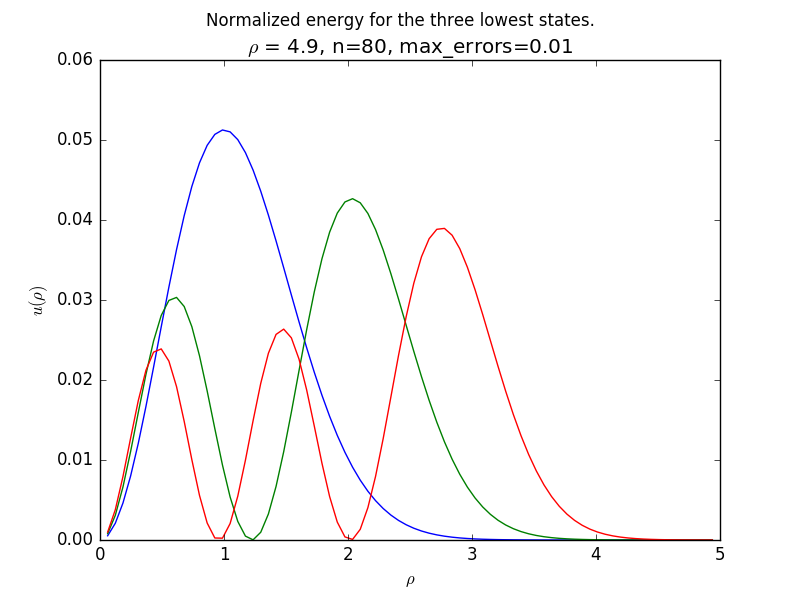
\includegraphics[width=0.45\textwidth]{eigenvector_rho49n80.png}

\caption{Normalized energy for the three lowest eigenvalues for a system with no repulsive Coulomb interaction with n=80}
\label{fig:Eigenvalue_states_n_80}
\end{figure}
\FloatBarrier



\FloatBarrier
\begin{figure}[!ht]
\centering
\FloatBarrier
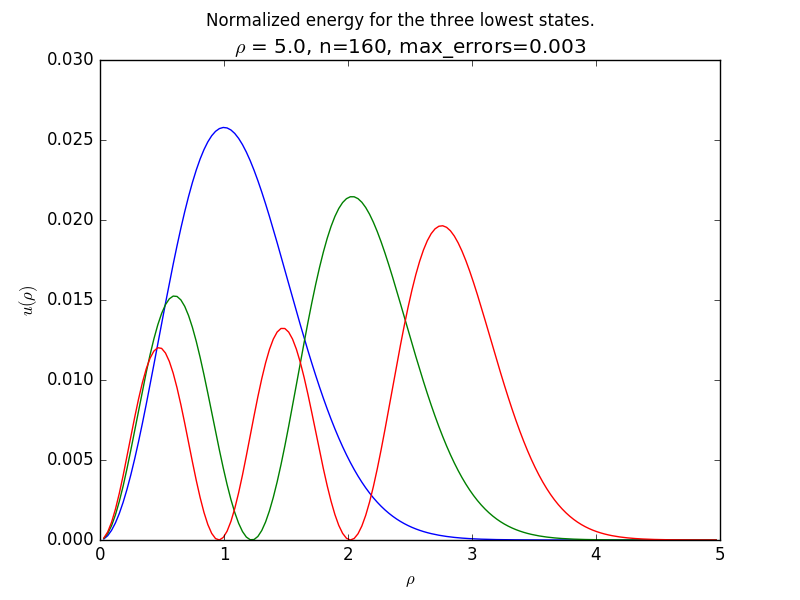
\includegraphics[width=0.45\textwidth]{eigenvector_rho49n160.png}

\caption{Normalized energy for the three lowest eigenvalues for a system with no repulsive Coulomb interaction with n=160}
\label{fig:Eigenvalue_states_n_160}
\end{figure}
\FloatBarrier


\FloatBarrier
\begin{figure}[!ht]
\centering
\FloatBarrier
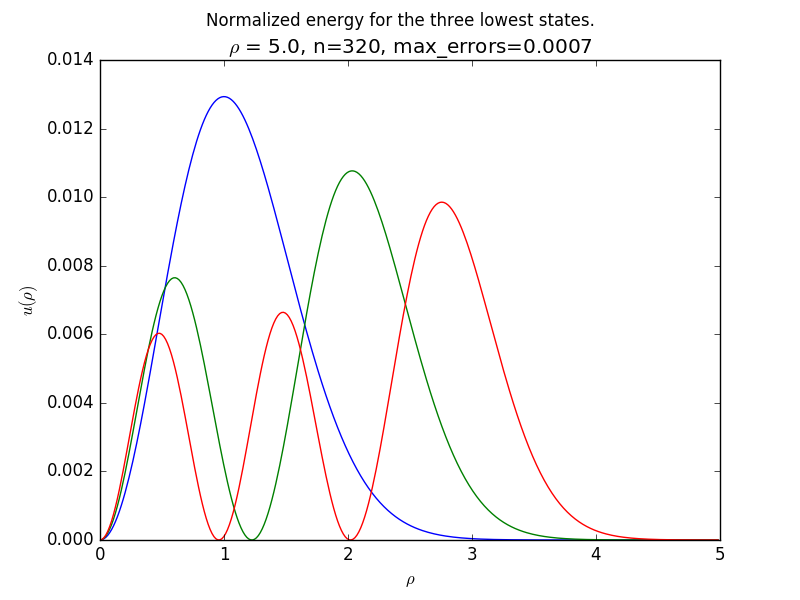
\includegraphics[width=0.45\textwidth]{eigenvector_rho49n320.png}

\caption{Normalized energy for the three lowest eigenvalues for a system with no repulsive Coulomb interaction with n=320}
\label{fig:Eigenvalue_states_n_320}
\end{figure}
\FloatBarrier


The function jacobi\_method finds the eigenvalues and eigenvectors for a symmetric matrix A through rotational transformations.
If the non-diagonal matrix elements are exactly 0, the diagonal elements are the eigenvalues. How many similarity transformations are needed to reach the accepted error tolerance for a given n is shown with different scalings in figure ~\ref{fig:Similarity_transformations_threshold_logy} and ~\ref{fig:Similarity_transformations_threshold_loglog}. The reference plot of $3n^2-5n$ is the theoretical value given in the lecture notes on the Jacobi method (Ch. 7.4, 23.10.17).

\FloatBarrier
\begin{figure}[!ht]
\centering
\FloatBarrier
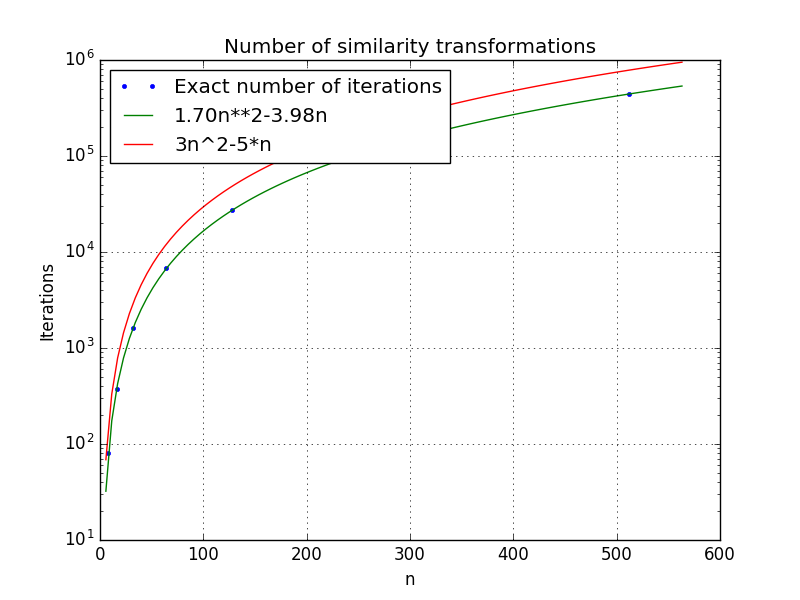
\includegraphics[width=0.45\textwidth]{num_iterations512n8logy.png}

\caption{Number of similarity transformations needed to reach the accepted error tolerance of $10^{-8}$ for the non-diagonal matrix elements, plotted with a logarithmic y-axis}
\label{fig:Similarity_transformations_threshold_logy}
\end{figure}
\FloatBarrier



\FloatBarrier
\begin{figure}[!ht]
\centering
\FloatBarrier
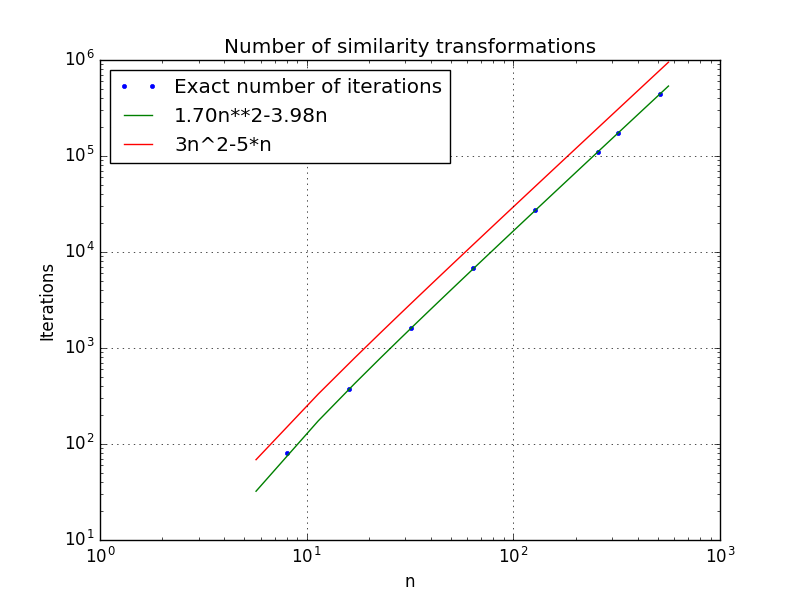
\includegraphics[width=0.45\textwidth]{num_iterations512n8loglog.png}

\caption{Number of similarity transformations needed to reach the accepted error tolerance of $10^{-8}$ for the non-diagonal matrix elements, plotted with a logarithmic x- and y-axis}
\label{fig:Similarity_transformations_threshold_loglog}
\end{figure}
\FloatBarrier


The convergence rate of the Jacobi method is poor. According to the lecture notes, one typically needs $3n^2-5n$. My calculations gave $1.7n^2-3.98n$, which is marginally better than the text book.



\section{Task 02c}
This section is about testing the code.

I set up three tests for the code, implemented with the program test\_project\_2.py given in my list of files to be found at my Github.

The tests are: \\
\begin{itemize}

\item test\_three\_first\_eigenvalues tests that the three first eigenvalues are correct within a tolerance of $10^{-4}$
\item test\_jacobi\_eigenvectors\_are\_orthogonal makes sure the eigenvectors are orthogonal
\item test\_jacobi\_solves\_eigen\_value\_eq makes sure the jacobi method solves the eigenvalue equation.

\end{itemize}


\section{Task 02d}
Schroedingers equation rewritten with a different potential to make it more general, allowing for a system with repulsive Coulomb interaction.\\


For figure ~\ref{fig:Eigenvalue_states_n_320_omega_100} the normalized energies are very similar compared to the non-interactive case from figure ~\ref{fig:Eigenvalue_states_n_320}. This is because the potential is very similar: Noninteractive case has potential $\rho^2$, whereas the interactive case has potential $\omega_r^2\rho^2+1/\rho$. For $\omega_r = 1$ the difference is only a term $1/\rho$, which is a small deviation for sufficiently large $\rho$. \\

The varying $\omega_r$ from figure ~\ref{fig:Eigenvalue_states_n_128_omega_1} to figure ~\ref{fig:Eigenvalue_states_n_320_omega_500} shows that the spikes of the energy increases with increasing $\omega_r$, which was expected since the potential is dependent on $\omega_r^2$. This means that the uncertainty for where the electrons are positioned is lower for larger $\omega_r$. At low values of $\omega_r$ the potential is spread over a wider range, giving the term $1/\rho$ more importance. To compensate for $\omega_r = 0.01$, I had to increase $\rho_{max}$ to 60  to fully capture the most probable position of the electrons. The theoretical approximate groundstate wavefunction is given right after equation 16a in the article by M.Taut 1993;  "Two electrons in an external oscillator potential", is plotted as reference with a dashed line.


\FloatBarrier
\begin{figure}[!ht]
\centering
\FloatBarrier
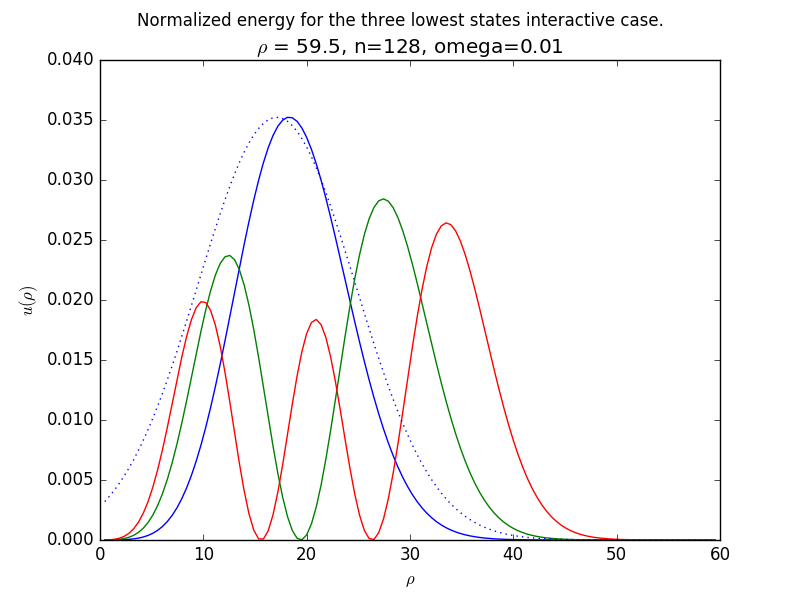
\includegraphics[width=0.45\textwidth]{eigenvector_rho595n128omega1}

\caption{Normalized energy for the three lowest eigenvalues for a system with repulsive Coulomb interaction with n=128 and $\omega_r$=0.01}
\label{fig:Eigenvalue_states_n_128_omega_1}
\end{figure}
\FloatBarrier


\FloatBarrier
\begin{figure}[!ht]
\centering
\FloatBarrier
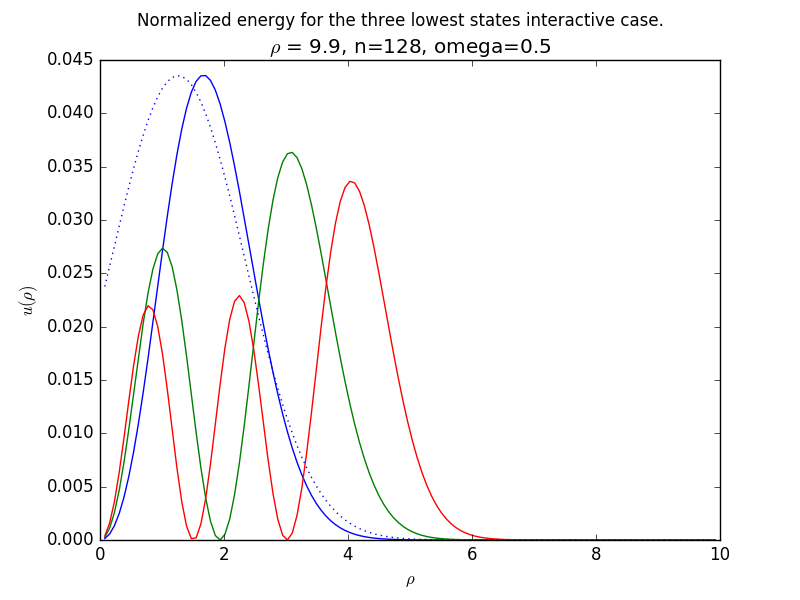
\includegraphics[width=0.45\textwidth]{eigenvector_rho99n128omega50.png}

\caption{Normalized energy for the three lowest eigenvalues for repulsive Coulomb interaction with n=128 and $\omega_r$=0.5}
\label{fig:Eigenvalue_states_n_128_omega_50}
\end{figure}
\FloatBarrier


\FloatBarrier
\begin{figure}[!ht]
\centering
\FloatBarrier
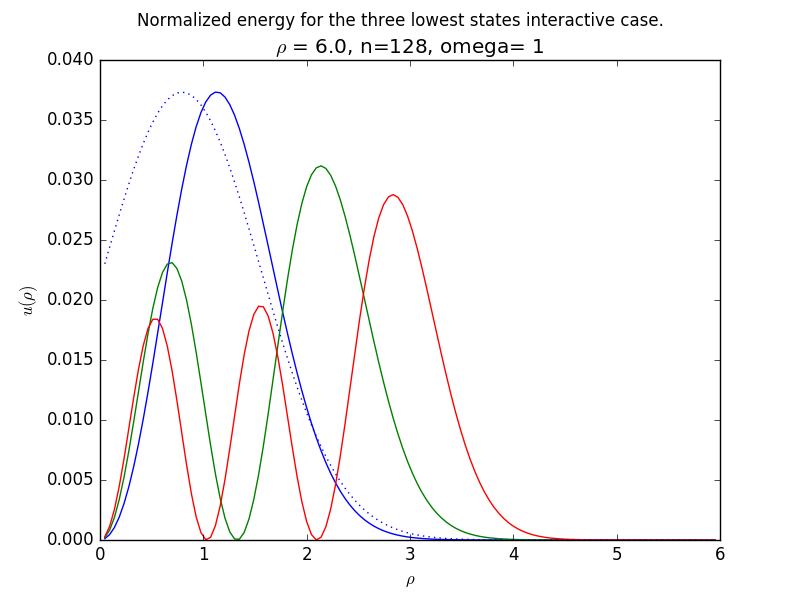
\includegraphics[width=0.45\textwidth]{eigenvector_rho59n128omega100.png}

\caption{Normalized energy for the three lowest eigenvalues for repulsive Coulomb interaction with n=128 and $\omega_r$=1}
\label{fig:Eigenvalue_states_n_320_omega_100}
\end{figure}
\FloatBarrier


\FloatBarrier
\begin{figure}[!ht]
\centering
\FloatBarrier
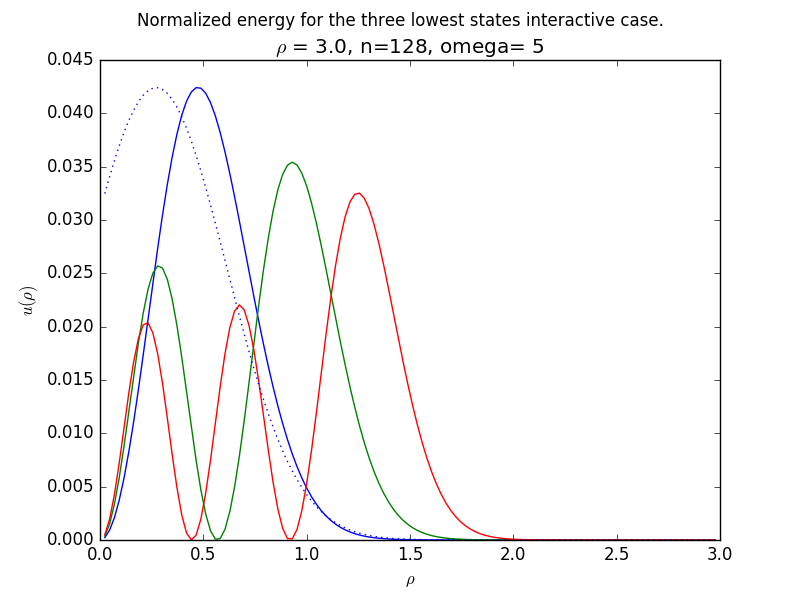
\includegraphics[width=0.45\textwidth]{eigenvector_rho29n128omega500.png}

\caption{Normalized energy for the three lowest eigenvalues for repulsive Coulomb interaction with n=128 and $\omega_r$=5}
\label{fig:Eigenvalue_states_n_320_omega_500}
\end{figure}
\FloatBarrier


\subsection{Comments}
I realize that I probably should have plotted only the lowest ground state for the four last plots. 